%%%%%%%%%%%%%%%%%%%%%%%%%%%%%%%%%%%%%%%%%%%%%%%%%%%%%%%%%%%%%%%%%%%%%%%%%%%%%%%

\section*{\large Exercício 4 - Espaço de Cullen-Frey e Distribuições de Probabilidades}
\addcontentsline{toc}{chapter}{\protect\numberline{}\large Exercício 4}%

Os resultados deste exercício se encontram na pasta \textbf{Exercise4}. Na pasta \textbf{familia1} estão as análises do grupo noise para $n$ = 8192, e na pasta \textbf{familia2} as análises do grupo colornoise para $n$ = 8192 e $\beta$ = 0.

\subsection*{4.1} 
\addcontentsline{toc}{section}{\protect\numberline{} 4.1}%

A análise desta Seção foi realizada com o script CullenFrey\_R\_Python.py.

\begin{figure}[ht!]
	%\caption{Série e histogramas.}
	\vspace{0mm}	% acrescentar o espaçamento vertical apropriado entre o título e a borda superior da figura
	\begin{center}
		\resizebox{12.5cm}{!}{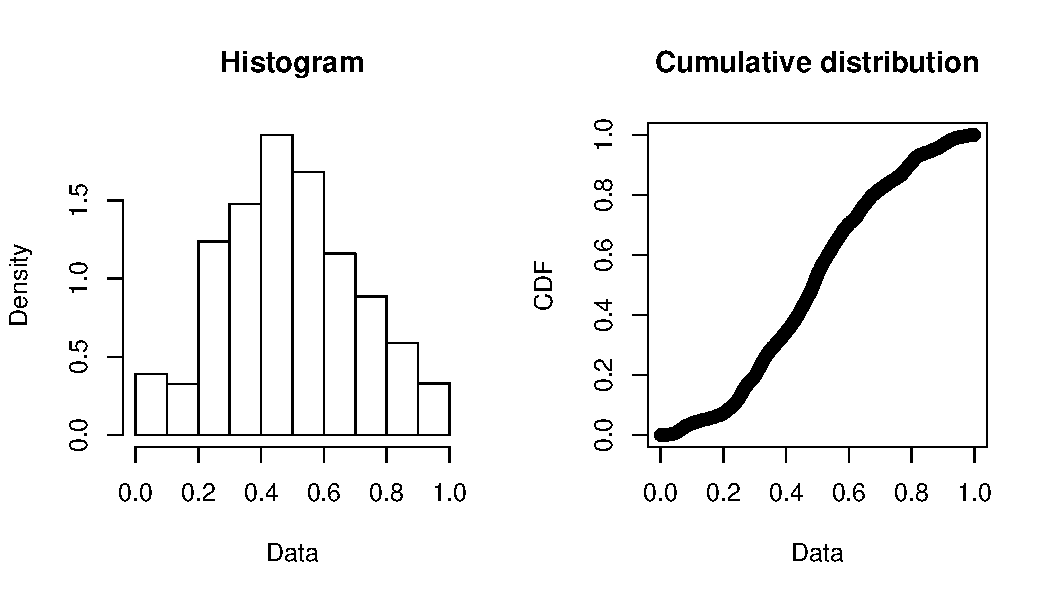
\includegraphics{Figuras/ex4/4_1/Exercicio4_1_fam1_histCDF.pdf}}		
	\end{center}
	\vspace{-2mm}	% acrescentar o espaçamento vertical apropriado entre a borda inferior da figura e a legenda ou a fonte quando não há legenda (o valor pode ser negativo para subir)
	\legenda{Figura 4.1.1: Histograma e CDF para a família 1 (noise) com $n$ = 8192.}	% legenda - para deixar sem legenda usar comando \legenda{} (nunca deve-se comentar o comando \legenda)
	\label{ex4_fig1}
	%\FONTE{}	% fonte consultada (elemento obrigatório, mesmo que seja produção do próprio autor)
\end{figure}

\begin{figure}[ht!]
	%\caption{Série e histogramas.}
	\vspace{0mm}	% acrescentar o espaçamento vertical apropriado entre o título e a borda superior da figura
	\begin{center}
		\resizebox{12.5cm}{!}{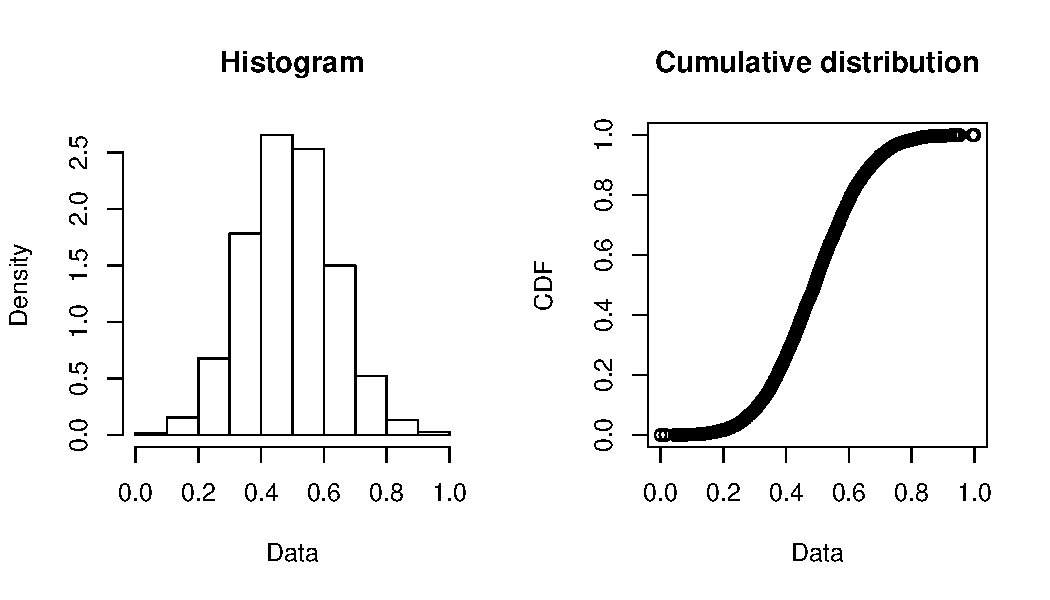
\includegraphics{Figuras/ex4/4_1/Exercicio4_1_fam2_histCDF.pdf}}		
	\end{center}
	\vspace{-2mm}	% acrescentar o espaçamento vertical apropriado entre a borda inferior da figura e a legenda ou a fonte quando não há legenda (o valor pode ser negativo para subir)
	\legenda{Figura 4.1.2: Histograma e CDF para a família 2 (colornoise) com $n$ = 8192 e $\beta$ = 0.}	% legenda - para deixar sem legenda usar comando \legenda{} (nunca deve-se comentar o comando \legenda)
	\label{ex4_fig2}
	%\FONTE{}	% fonte consultada (elemento obrigatório, mesmo que seja produção do próprio autor)
\end{figure}

\begin{figure}[ht!]
	%\caption{Série e histogramas.}
	\vspace{-3mm}	% acrescentar o espaçamento vertical apropriado entre o título e a borda superior da figura
	\begin{center}
		\resizebox{10.cm}{!}{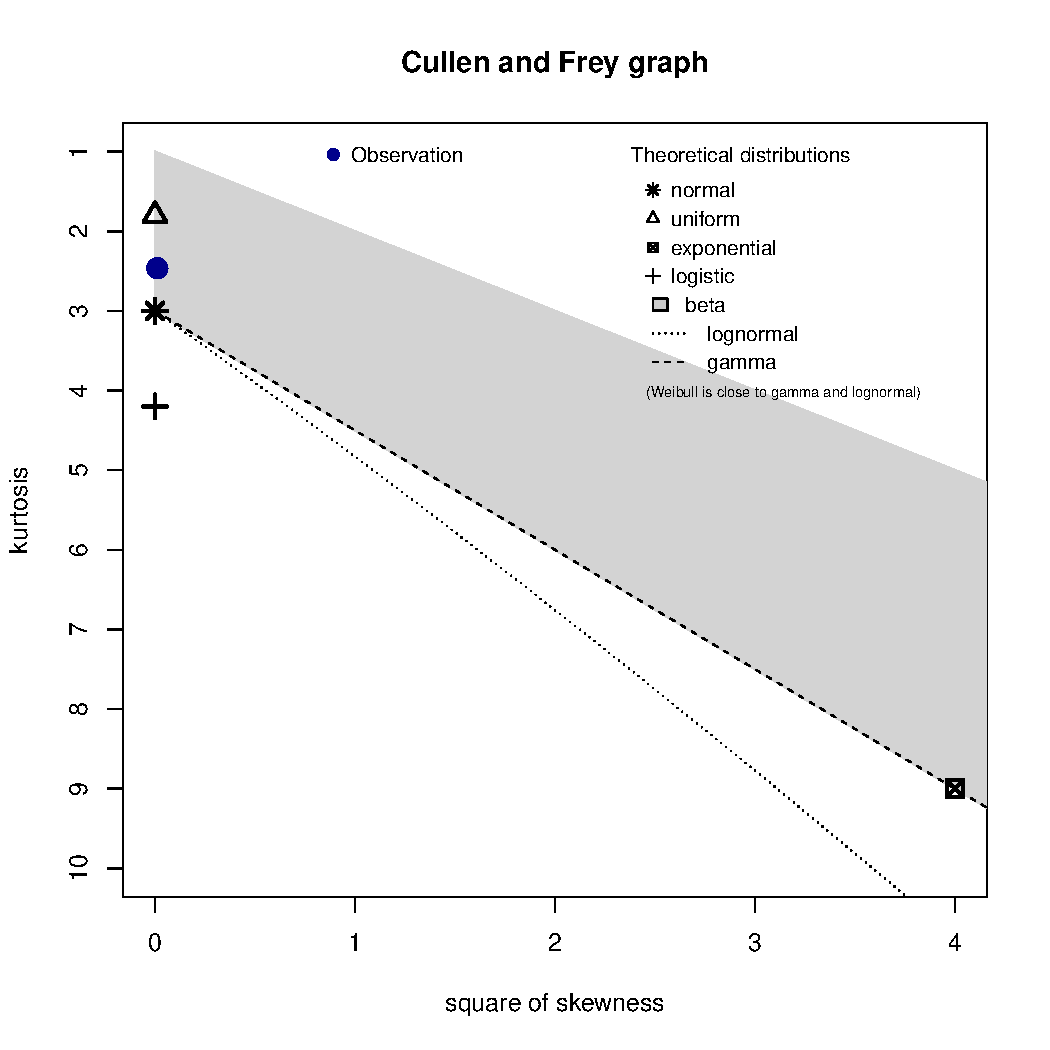
\includegraphics{Figuras/ex4/4_1/Exercicio4_1_fam1_CullenFrey.pdf}}		
	\end{center}
	\vspace{-3mm}	% acrescentar o espaçamento vertical apropriado entre a borda inferior da figura e a legenda ou a fonte quando não há legenda (o valor pode ser negativo para subir)
	\legenda{Figura 4.1.3: Resultado da análise Cullen and Frey para a família 1 (noise).}	% legenda - para deixar sem legenda usar comando \legenda{} (nunca deve-se comentar o comando \legenda)
	\label{ex4_fig3}
	%\FONTE{}	% fonte consultada (elemento obrigatório, mesmo que seja produção do próprio autor)
\end{figure}

\begin{figure}[ht!]
	%\caption{Série e histogramas.}
	\vspace{-3mm}	% acrescentar o espaçamento vertical apropriado entre o título e a borda superior da figura
	\begin{center}
		\resizebox{10.cm}{!}{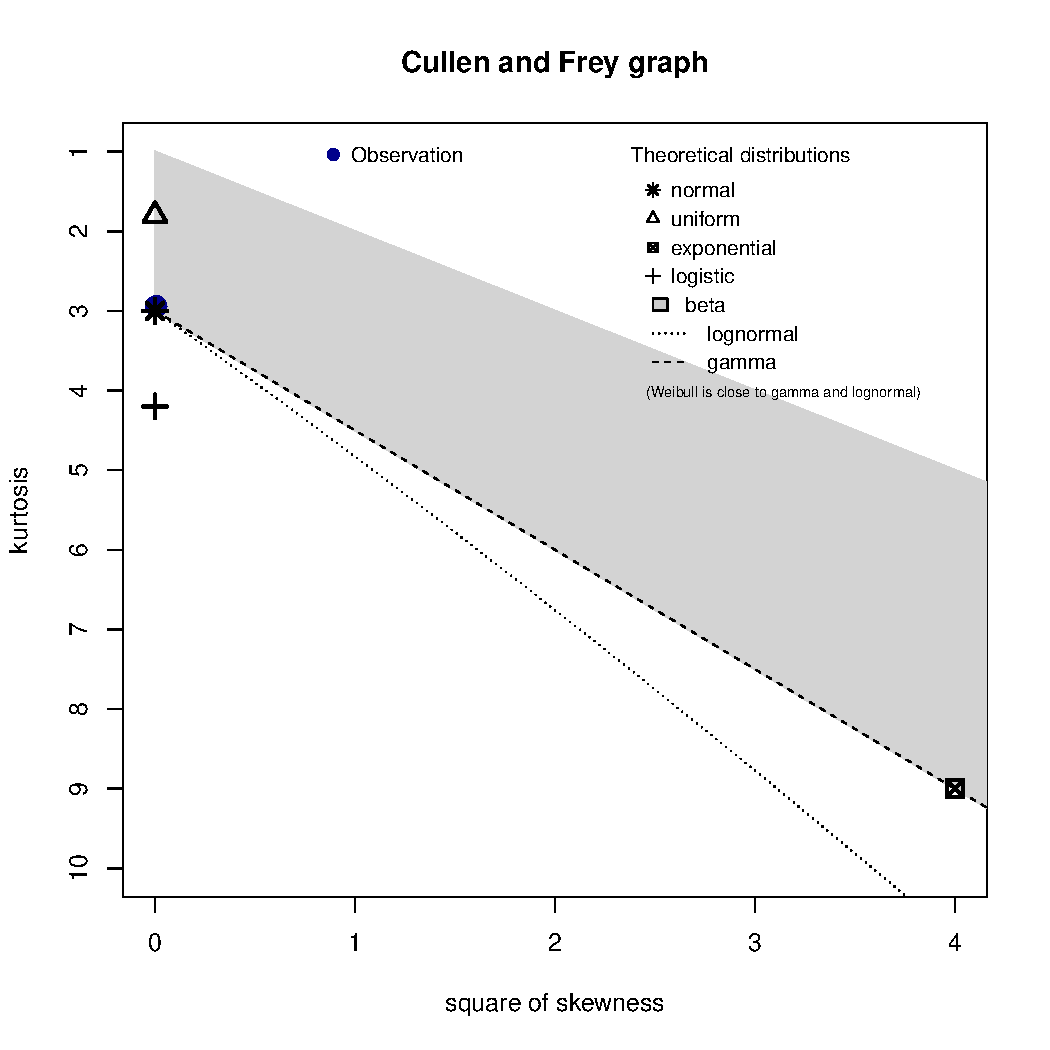
\includegraphics{Figuras/ex4/4_1/Exercicio4_1_fam2_CullenFrey.pdf}}		
	\end{center}
	\vspace{-3mm}	% acrescentar o espaçamento vertical apropriado entre a borda inferior da figura e a legenda ou a fonte quando não há legenda (o valor pode ser negativo para subir)
	\legenda{Figura 4.1.4: Resultado da análise Cullen and Frey para a família 2 (pmnoise).}	% legenda - para deixar sem legenda usar comando \legenda{} (nunca deve-se comentar o comando \legenda)
	\label{ex4_fig4}
	%\FONTE{}	% fonte consultada (elemento obrigatório, mesmo que seja produção do próprio autor)
\end{figure}

%%%%%%%%%%%%%%%%%%%%%%%%%%%%%%%%%%%%%%%%%%% 4.2 %%%%%%%%%%%%%%%%%%%%%%%%%%%%%%%%%%%%%%%%%%%%%%%%
\clearpage
\subsection*{4.2}
\addcontentsline{toc}{section}{\protect\numberline{} 4.2}%

Todos os resultados desta Seção forma gerados com os scripts Distribution\_Fitter\_Python.py e Distribution\_Fitter\_R.py.

%%%%%%%%%%%%%%%%% familia 1 %%%%%%%%%%%%%%%%%%%%%

\subsubsection*{Primeira família}

\begin{figure}[ht!]
	%\caption{Série e histogramas.}
	\vspace{0mm}	% acrescentar o espaçamento vertical apropriado entre o título e a borda superior da figura
	\begin{center}
		\resizebox{13cm}{!}{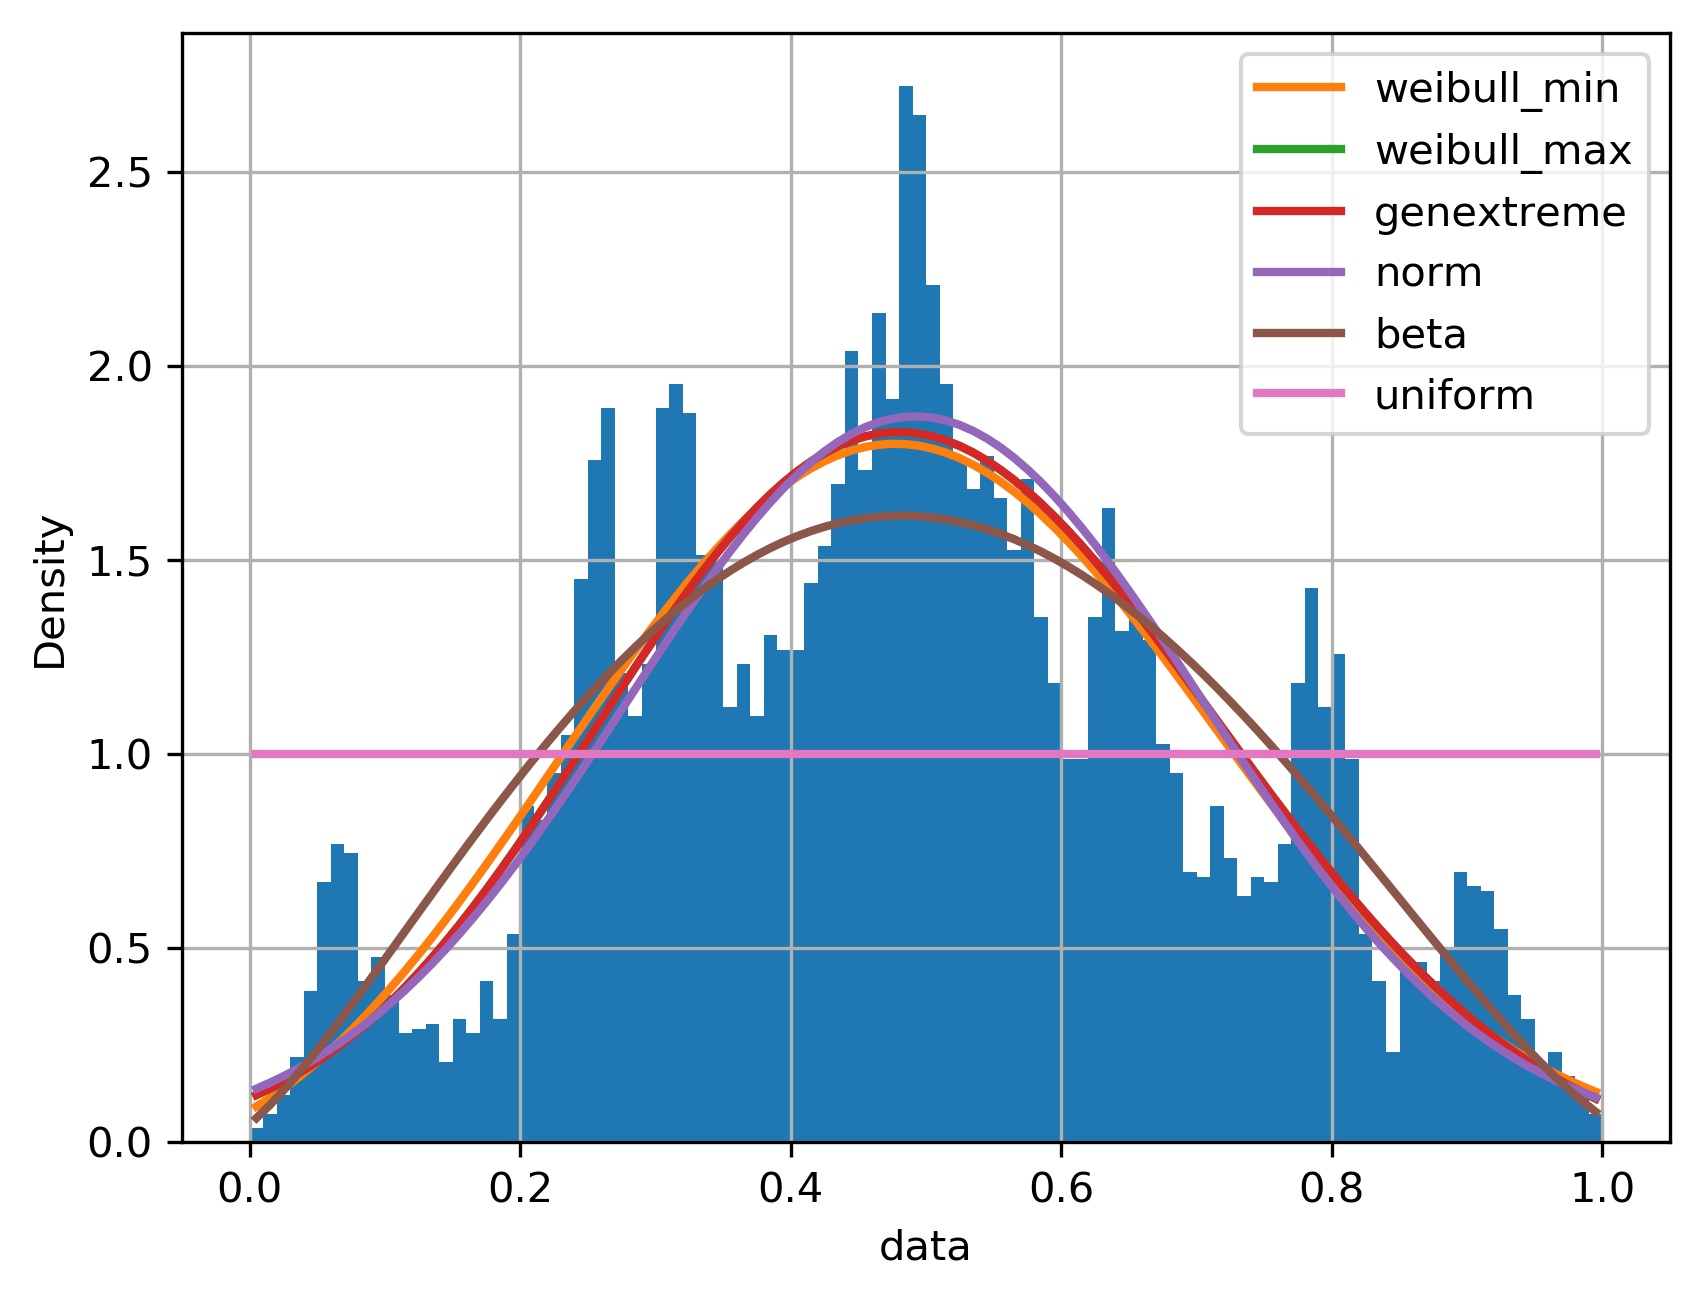
\includegraphics{Figuras/ex4/4_2/Exercicio4_2_fam1_Python_fits.jpg}}		
	\end{center}
	\vspace{-2mm}	% acrescentar o espaçamento vertical apropriado entre a borda inferior da figura e a legenda ou a fonte quando não há legenda (o valor pode ser negativo para subir)
	\legenda{Figura 4.2.1: Resultado do ajuste de 6 distribuições diferentes, incluindo GEV, na família noise. Foi utilizado o script Distribution\_Fitter\_Python.py para este plot.}	% legenda - para deixar sem legenda usar comando \legenda{} (nunca deve-se comentar o comando \legenda)
	\label{ex4_fig8}
	%\FONTE{}	% fonte consultada (elemento obrigatório, mesmo que seja produção do próprio autor)
\end{figure}

Abaixo o resultado do benchmark gerado automaticamente pelo script Distribution\_Fitter\_Python.py, presente no arquivo \textit{Exercicio4\_2\_fam1\_Python\_fits.txt}, que permite avaliar a performance de cada distribuição no ajuste empregado. Observa-se que a \texttt{weibull} foi a distribuição com menor erro.

\begin{figure}[ht!]
	%\caption{Série e histogramas.}
	\vspace{0mm}	% acrescentar o espaçamento vertical apropriado entre o título e a borda superior da figura
	%\begin{center}
		\resizebox{12cm}{!}{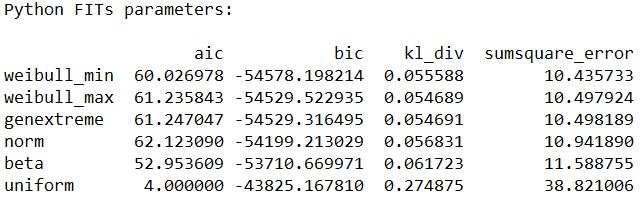
\includegraphics{Figuras/ex4/4_2/Exercicio4_2_fam1_Python_fits_params.jpg}}		
	%\end{center}
	\vspace{-2mm}	% acrescentar o espaçamento vertical apropriado entre a borda inferior da figura e a legenda ou a fonte quando não há legenda (o valor pode ser negativo para subir)
	%\legenda{Figura 4.2.4:.}	% legenda - para deixar sem legenda usar comando \legenda{} (nunca deve-se comentar o comando \legenda)
	%\label{ex4_fig8}
	%\FONTE{}	% fonte consultada (elemento obrigatório, mesmo que seja produção do próprio autor)
\end{figure}

\begin{figure}[ht!]
	%\caption{Série e histogramas.}
	\vspace{-3mm}	% acrescentar o espaçamento vertical apropriado entre o título e a borda superior da figura
	\begin{center}
		\resizebox{12cm}{!}{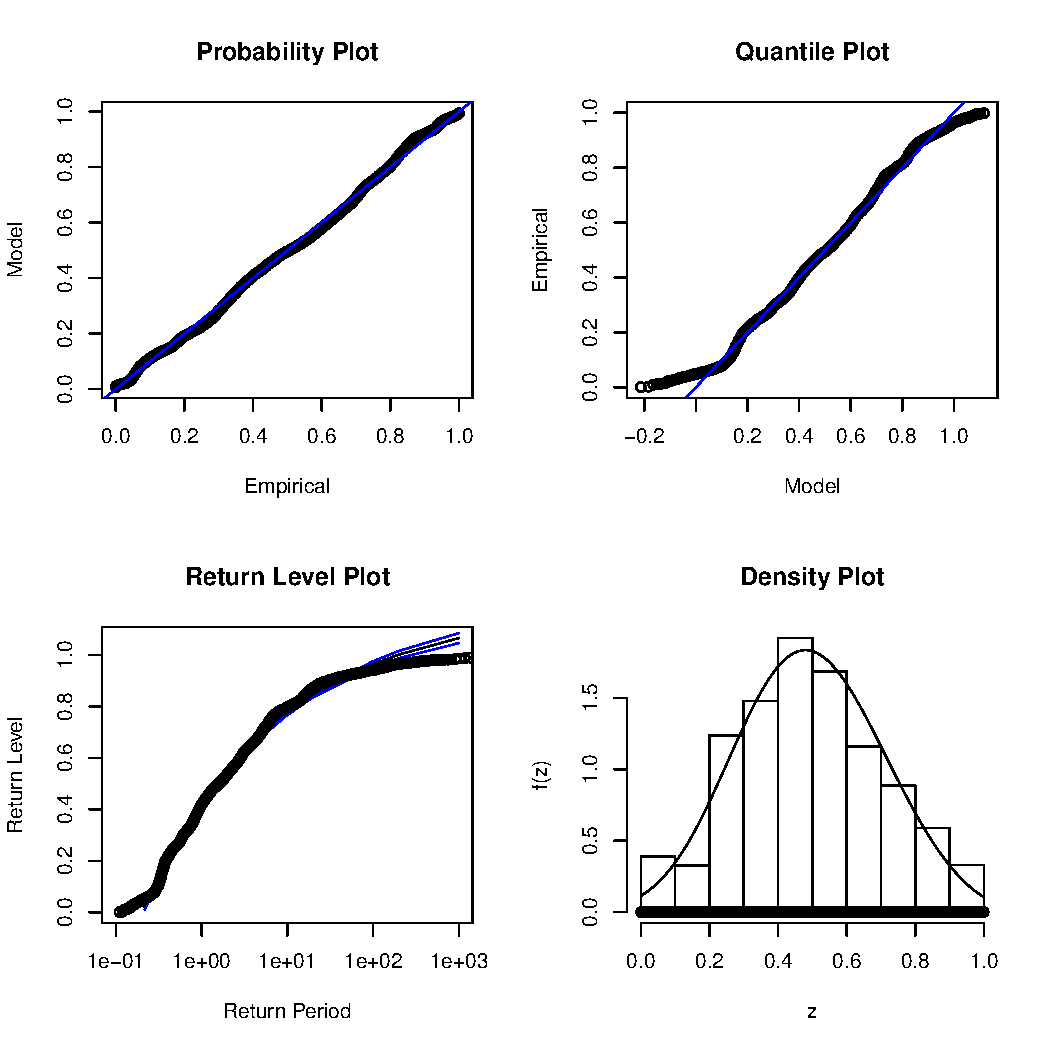
\includegraphics{Figuras/ex4/4_2/Exercicio4_2_fam1_GEV.pdf}}		
	\end{center}
	\vspace{-3mm}	% acrescentar o espaçamento vertical apropriado entre a borda inferior da figura e a legenda ou a fonte quando não há legenda (o valor pode ser negativo para subir)
	\legenda{Figura 4.2.2: Resultado do ajuste da GEV com o script Distribution\_Fitter\_R.py. Um ajuste das mesmas distribuições da Figura 4.2.1 foi gerado, mas essa figura ilustra apenas a performance da GEV com o script com ambiente R em Python, que inclui plots dos quantis teóricos vs os empíricos, e das probabilidades teóricas vs as empíricas, além da curva da GEV sobre o histograma da série.}	% legenda - para deixar sem legenda usar comando \legenda{} (nunca deve-se comentar o comando \legenda)
	\label{ex4_fig6}
	%\FONTE{}	% fonte consultada (elemento obrigatório, mesmo que seja produção do próprio autor)
\end{figure}
%que indica a convergência do ajuste da GEV e 
Abaixo o resultado do benchmark gerado automaticamente pelo script Distribution\_Fitter\_R.py para o ajuste de uma GEV, presente no arquivo \textit{Exercicio4\_2\_fam1\_GEV\_params.txt}, com o resultado dos parâmetros da GEV via \texttt{MLE} (Maximum Likelihood Estimation) e seus respectivos erros.  

\begin{figure}[ht!]
	%\caption{Série e histogramas.}
	\vspace{0mm}	% acrescentar o espaçamento vertical apropriado entre o título e a borda superior da figura
	%\begin{center}
		\resizebox{13.5cm}{!}{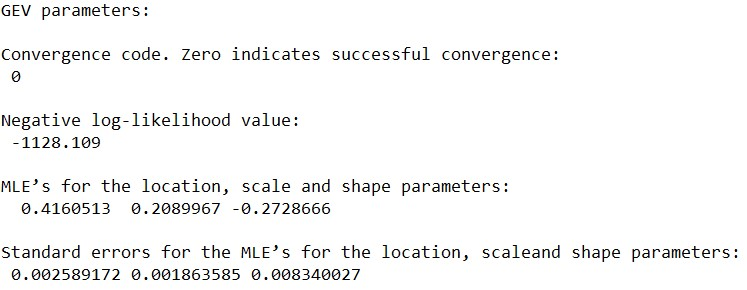
\includegraphics{Figuras/ex4/4_2/Exercicio4_2_fam1_GEV_params.jpg}}		
	%\end{center}
	\vspace{-2mm}	% acrescentar o espaçamento vertical apropriado entre a borda inferior da figura e a legenda ou a fonte quando não há legenda (o valor pode ser negativo para subir)
	%\legenda{Figura 4.2.3:.}	% legenda - para deixar sem legenda usar comando \legenda{} (nunca deve-se comentar o comando \legenda)
	\label{ex4_fig7}
	%\FONTE{}	% fonte consultada (elemento obrigatório, mesmo que seja produção do próprio autor)
\end{figure}

%%%%%%%%%%%%%%%%%%%%%%% familia 2 %%%%%%%%%%%%%%%%%%%%%%%%
\clearpage
\subsubsection*{Segunda família}

\begin{figure}[ht!]
	%\caption{Série e histogramas.}
	\vspace{0mm}	% acrescentar o espaçamento vertical apropriado entre o título e a borda superior da figura
	\begin{center}
		\resizebox{12cm}{!}{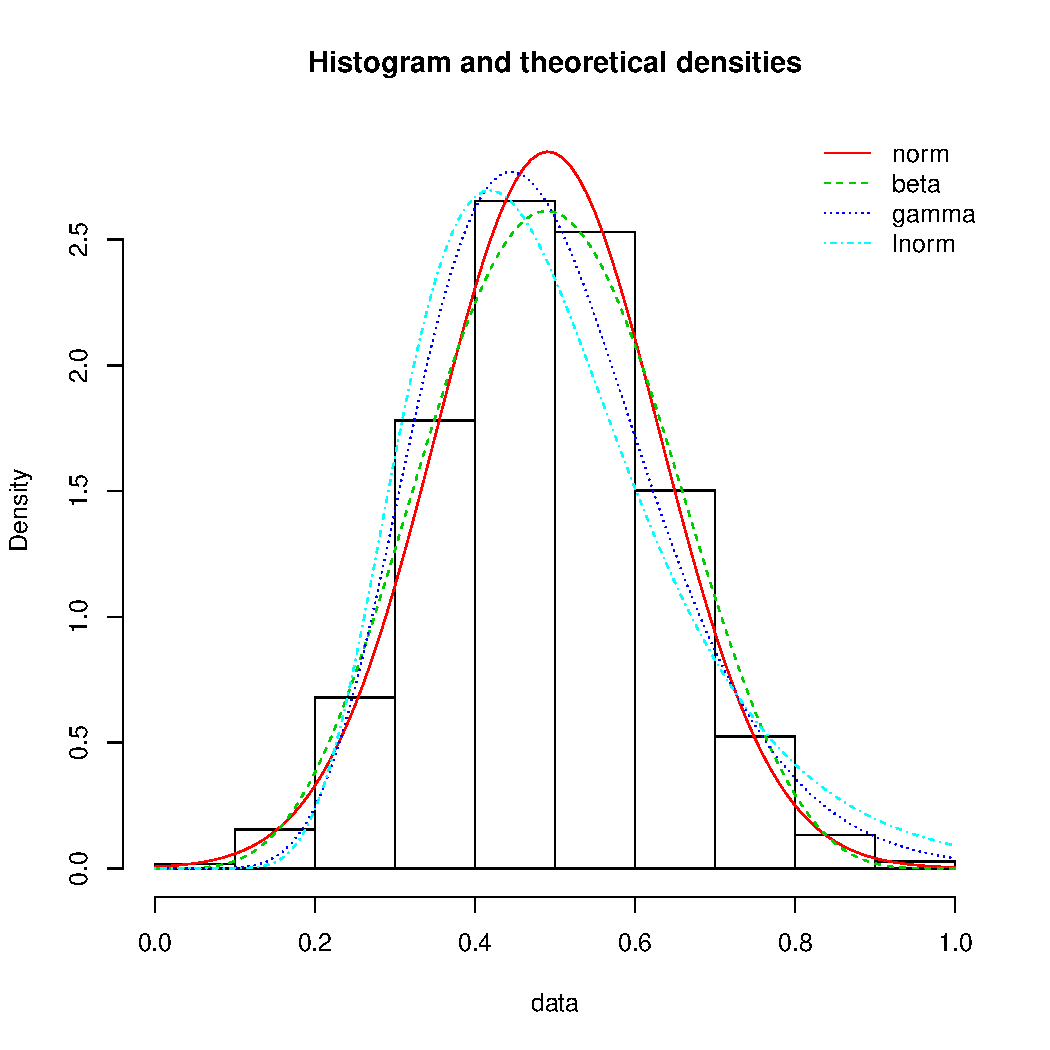
\includegraphics{Figuras/ex4/4_2/Exercicio4_2_fam2_fitComp.pdf}}		
	\end{center}
	\vspace{-2mm}	% acrescentar o espaçamento vertical apropriado entre a borda inferior da figura e a legenda ou a fonte quando não há legenda (o valor pode ser negativo para subir)
	\legenda{Figura 4.2.3: Resultado do ajuste de 4 distribuições diferentes na família pmnoise. Foi utilizado o script Distribution\_Fitter\_R.py para este plot. Não foi ajustada uma GEV para esta família.}	% legenda - para deixar sem legenda usar comando \legenda{} (nunca deve-se comentar o comando \legenda)
	\label{ex4_fig9}
	%\FONTE{}	% fonte consultada (elemento obrigatório, mesmo que seja produção do próprio autor)
\end{figure}

Abaixo o resultado do benchmark gerado automaticamente pelo script Distribution\_Fitter\_R.py, presente no arquivo \textit{Exercicio4\_2\_fam1\_gof.txt}, com o resultado dos ajustes através do método \texttt{mle} (maximum likelihood estimation), que é o padrão do código. Observa-se que a distribuição \texttt{normal} foi a de melhor performance.

\begin{figure}[ht!]
	%\caption{Série e histogramas.}
	\vspace{0mm}	% acrescentar o espaçamento vertical apropriado entre o título e a borda superior da figura
	%\begin{center}
		\resizebox{14cm}{!}{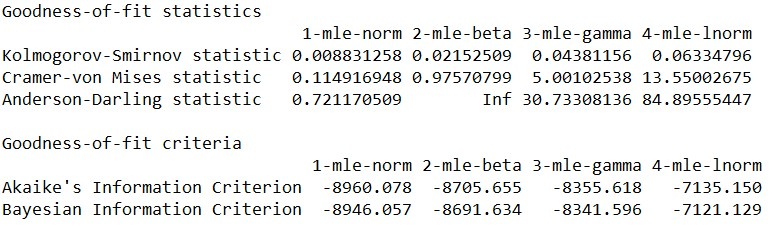
\includegraphics{Figuras/ex4/4_2/Exercicio4_2_fam2_gof.jpg}}		
	%\end{center}
	\vspace{-2mm}	% acrescentar o espaçamento vertical apropriado entre a borda inferior da figura e a legenda ou a fonte quando não há legenda (o valor pode ser negativo para subir)
	%\legenda{Figura 4.2.6:.}	% legenda - para deixar sem legenda usar comando \legenda{} (nunca deve-se comentar o comando \legenda)
	\label{ex4_fig10}
	%\FONTE{}	% fonte consultada (elemento obrigatório, mesmo que seja produção do próprio autor)
\end{figure}

